\documentclass{article}
\usepackage[
paperwidth = 12.5cm, 
paperheight=15cm,
textwidth = 12.5cm,
textheight =15cm,
nohead,
nofoot,
nomarginpar,         
margin=0mm]{geometry}
\usepackage{amsmath,amsfonts,amssymb}
\usepackage{tikz,pgfplots}
\usetikzlibrary{arrows,arrows.meta,bending,calc,decorations,shadings,shadows,shapes,shapes.arrows,shapes.geometric}
\usetikzlibrary{calc,fadings,decorations.pathreplacing}
\usepgfplotslibrary{units,fillbetween,groupplots,colorbrewer}
\usetikzlibrary{pgfplots.colorbrewer,}
\usepackage{pgfplotstable}
\usetikzlibrary{3d,spy}
\usepgfmodule{plot}
\usepackage{scalerel}
\usepackage{graphicx}
\usepackage{tikz-dimline}
\usepackage{epstopdf}
\epstopdfsetup{outdir=out/,suffix=-generated}
\definecolor{As}{RGB}{255,255,0}
\definecolor{Al}{RGB}{173,216,230}
\definecolor{Ga}{RGB}{0,128,150}

\definecolor{background}{RGB}{77,77,77}

\definecolor{plane100}{RGB}{0,178,69}
\definecolor{plane010}{RGB}{0,255,208}

\newcommand*{\xMin}{0}%
\newcommand*{\xMax}{14}%
\newcommand*{\yMin}{-7}%
\newcommand*{\yMax}{0}%

\begin{document}
	\thispagestyle{empty}
\begin{tikzpicture}[remember picture,overlay]


\node [draw=blue!60,circle,inner sep=-0.3mm,align=center,ball color=cyan,scale=8,opacity=0](c0) at ([xshift=-4cm]current page.center) {$\displaystyle C_{2v}$};


\node [draw=blue!60,circle,inner sep=0mm,inner sep=-3mm,line width=.5mm](c1) at ([xshift=5cm]c0.east) {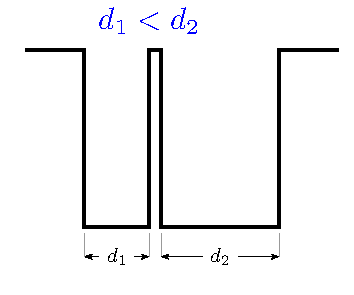
\includegraphics[scale=0.7]{out/acqws-2.pdf}};
\def\arcccu{235}
\def\arcccd{55}

\draw[color=blue!60,right color=blue,middle
color=blue,fill opacity=0.3,line width=.5mm,draw opacity=1,rounded corners,inner sep=0mm]  
(c0.south east) to [bend left] (c1.south west)  arc (225:140:2.3) -- 
(c1.north west) to [bend left] (c0.north east) arc (45:-45:2.25);


\node [draw=blue!60,circle,inner sep=0mm,inner sep=-3mm,line width=.5mm](c2) at ([xshift=2.5cm,yshift=3.5cm]c0.north east) {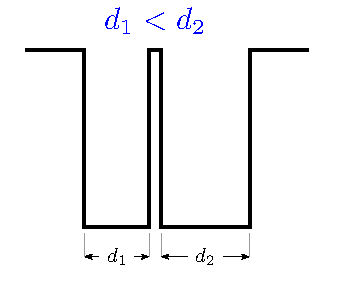
\includegraphics[scale=0.7]{out/acqws-1}};

\draw[color=blue!60,right color=blue,middle
color=blue,fill opacity=0.3,line width=.5mm,draw opacity=1,rounded corners,inner sep=0mm]  
(c0.east) to [bend left] (c2.south) arc (270:170:2.3)--
(c2.west) to [bend left] (c0.north) arc (90:0:2.3);

\node [draw=red!60,circle,inner sep=0mm,inner sep=-3mm,line width=.5mm](c3) at ([xshift=2.5cm,yshift=-3.5cm]c0.south east) {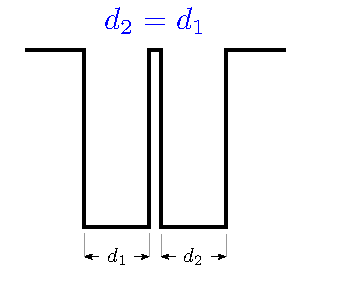
\includegraphics[scale=0.7]{out/scqws}};


\draw[color=red!60,right color=red,middle
color=red,fill opacity=0.3,line width=.5mm,draw opacity=1,rounded corners,inner sep=0mm]  
(c0.east) to [bend right] (c3.north) arc (90:185:2.3)--
(c3.west) to [bend right] (c0.south) arc (270:360:2.3);


\begin{scope}
\node [draw=blue!60,circle,inner sep=-0.3mm,align=center,ball color=cyan,scale=8,opacity=1](c0) at ([xshift=-4cm]current page.center) {$\displaystyle C_{2v}$};
\clip ([xshift=-4cm]current page.center) circle (2.25cm) node [opacity=0.2] {\includegraphics[scale=0.1]{/media/labfiles/ruco/phd-ssp/scripts/symmetry/acqws-symmetry1-out.pdf}};	
\end{scope}






\end{tikzpicture}
	
	


\end{document}